\section{Introduction}


\begin{frame}{What is robust optimisation}

	An alternative paradigm for taking uncertainty into account:
	\begin{itemize}
		\item Permeated by the notion of \alert{worst-case};
		\item Control of the degree of \alert{conservatism};	
		\item Parallels with \alert{chance constraints} and \alert{risk measures}.
	\end{itemize}
	
	\pause
	In robust optimisation, \alert{feasibility} is the key concern
	\begin{itemize}
		\item Can be extended to objective function performance requirements;
		\item May or may not be \alert{scenario-based};
		\item Static v. adaptable: the presence of \alert{recourse decisions};
		\item Exception: distributionally robust optimisation.	
	\end{itemize}
	
\end{frame}

\begin{frame}{Robust optimisation approaches}
	
	
	\begin{columns}
	\column{0.45\textwidth}
	The key notion in robust optimisation is tie to that of an \alert{uncertainty set}
	\begin{itemize}
		\item The ``region'' $U$ within the uncertainty support $\Xi$ within which \alert{parameter realisation} does not turn the solution infeasible;
		\item Tractability is closely tied to the \alert{geometry} of such uncertainty sets.
	\end{itemize}
	
	\pause
	\column{0.45\textwidth}
	\vspace{-12pt}
	\begin{align*}
		\mini_x & c^\top x \\
		\text{s.t.: } & Ax \le b \\
		& x \in X \\
		&\quad \Downarrow \\
		\mini_x & c^\top x \\
		\text{s.t.: } & A(\eta)x \le b, \ \forall \eta \in U \subseteq \Xi \\
		& x \in X \\
		&\quad \Downarrow \\
		\mini_x & c^\top x \\
		\text{s.t.: } & \max_{\eta \in U \subseteq \Xi}A(\eta)x \le b \\
			& x \in X.
	\end{align*}
	\end{columns}

\end{frame}


\section{Robust optimisation}


\begin{frame}{Robust counterparts}

	Let $\tilde{a}_{ij} \in J_i$ be the \alert{uncertain elements} in the matrix $A_{m \times n}$ 
	\vspace{-6pt}
	\begin{itemize}
		\item Random variables $\tilde{a}_{ij}$ with ``central value'' $a_{ij}$ and ``maximum deviation'' $\hat{a}_{ij}$;
		\item symmetric and with bounded support $\tilde{a}_{ij} \in \brackets{a_{ij} - \hat{a}_{ij} , a_{ij} + \hat{a}_{ij}}$.
	\end{itemize}
	
	\pause
	Let $\eta_{ij} = \frac{(\tilde{a}_{ij} - a_{ij})}{\hat{a}_{ij}}$. Thus $\eta_{ij} \in \brackets{-1,1}$ and follows the \alert{same distribution} as $\tilde{a}_{ij}$, but centred in zero and scaled. 
 
	Our robust counterpart%
	\footnote{Assuming, w.l.g., $a_{ij} \ge 0$, $\forall i \in [m], \forall j \in [n]$}
	%
	 is the following \alert{bilevel} problem:
	\begin{equation} \tag{RC}
		\begin{aligned}
			\mini_x & c^\top x \\
			\text{s.t.: } & a_{ij}x_j + \max_{\eta_i \in U_i} \braces{\sum_{j \in J_i}\eta_{ij}\hat{a}_{ij}x_j} \le b_i, \forall i \in [m] \\
			& x_j \ge 0, \ \forall j \in [n].			
		\end{aligned}
	\end{equation}
\end{frame}

\begin{frame}{Uncertainty set geometries}{Box uncertainty set \cite{soyster1973convex}}

	\begin{itemize}
		\item \alert{Maximum} protection level;
		\item All parameters take their worst-possible value;
		\item Simple, but highly conservative.
	\end{itemize}

	The \alert{uncertainty set} is
	$$
		U_i = \braces{\eta_i : ||\eta_i||_1 \le |J_i|} \equiv \braces{\eta_{ij} : |\eta_{ij}| \le 1, \forall j \in J_i}
	$$
	\pause
	The \alert{lower-level problem} becomes
	\begin{equation*}
		\maxi_{\eta_i \in U_i}\braces{\sum_{j \in J_i} \eta_{ij}\hat{a}_{ij}x_j : |\eta_{ij}| \le 1, \forall j \in J_i} = \sum_{j \in J_i}\hat{a}_{ij}x_j.
	\end{equation*}	

\end{frame}

\begin{frame}{Uncertainty set geometries}{Box uncertainty set \cite{soyster1973convex}}
	\centering 
	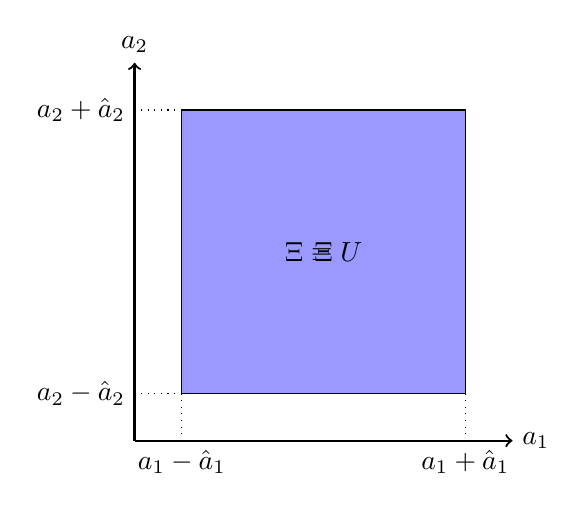
\begin{tikzpicture}[scale = 1.2]
		% Uncertainty set
		\uncover<2->{\filldraw[fill=blue!40!white] (0.5,0.5) rectangle (3.5,3.5);}
%		\draw[help lines] (0,0) grid (4,4);
		\draw[dashed] (0.5,0.5) rectangle (3.5,3.5);
		\draw[thick, ->] (0,0) -- (0,4);
		\draw[thick, ->] (0,0) -- (4,0);
		\node[right] at (4,0) {$a_1$};
		\node[above] at (0,4) {$a_2$}; 
		\draw[dotted] (0.5,0.5) -- (0.5,0) node[below] {$a_1 - \hat{a}_1$}; 
		\draw[dotted] (3.5,0.5) -- (3.5,0) node[below] {$a_1 + \hat{a}_1$};
		\draw[dotted] (0.5,0.5) -- (0,0.5) node[left] {$a_2 - \hat{a}_2$}; 
		\draw[dotted] (0.5,3.5) -- (0,3.5) node[left] {$a_2 + \hat{a}_2$};
		\uncover<1>{\node at (2,2) {$\Xi$};}
		\uncover<2->{\node at (2,2) {$\Xi \equiv U$};}
	\end{tikzpicture}
	
\end{frame}


\begin{frame}{Uncertainty set geometries}{Ellipsoidal uncertainty set \cite{ben1999robust}}

	\begin{itemize}
		\item \alert{Softens} extreme-case protection;
		\item Parametrically controlled;
		\item Leads to smooth sets;
		\item (MI)SOCPs which are more computationally demanding.
	\end{itemize}

	The \alert{uncertainty set} is
		$$
			U_i = \braces{\eta_{i} : ||\eta_{i}||_2 \le \Gamma} \equiv \braces{\eta_{ij} : \sum_{j \in J_i} \eta_{ij}^2 \le \Gamma^2, \forall j \in J_i}
		$$
	\pause	
	The \alert{lower-level problem} becomes
	\begin{equation*}
		\maxi_{\eta_i \in U_i}\braces{\sum_{j \in J_i} \eta_{ij}\hat{a}_{ij}x_j : \sum_{j \in J_i} \eta_{ij}^2 \le \Gamma^2, \forall j \in J_i}.
	\end{equation*}
	
\end{frame}


\begin{frame}{Uncertainty set geometries}{Ellipsoidal uncertainty set \cite{ben1999robust}}

	Again, this uncertainty set has a \alert{closed-form} solution:
	\begin{equation*}
		\begin{aligned}
			  & \maxi_{\eta_i \in U_i}\braces{\sum_{j \in J_i} \eta_{ij}\hat{a}_{ij}x_j : \sum_{j \in J_i} \eta_{ij}^2 \le \Gamma^2, \forall j \in J_i} \\
			= & \maxi_{\eta_i \in U_i}\braces{\sqrt{\left(\sum_{j \in J_i} \eta_{ij}\hat{a}_{ij}x_j\right)^2} : \sum_{j \in J_i} \eta_{ij}^2 \le \Gamma^2, \forall j \in J_i} \\
			= & \maxi_{\eta_i \in U_i}\braces{\sqrt{\left(\sum_{j \in J_i} \eta_{ij}\right)^2\left(\sum_{j \in J_i}\hat{a}_{ij}x_j\right)^2} : \sum_{j \in J_i} \eta_{ij}^2 \le \Gamma^2, \forall j \in J_i} \\	
			= & \Gamma \sqrt{\sum_{j \in J_i} \hat{a}_{ij}^2 x_j^2}
		\end{aligned}
		\end{equation*}
		
\end{frame}


\begin{frame}{Uncertainty set geometries}{Ellipsoidal uncertainty set \cite{ben1999robust}}

	\centering
	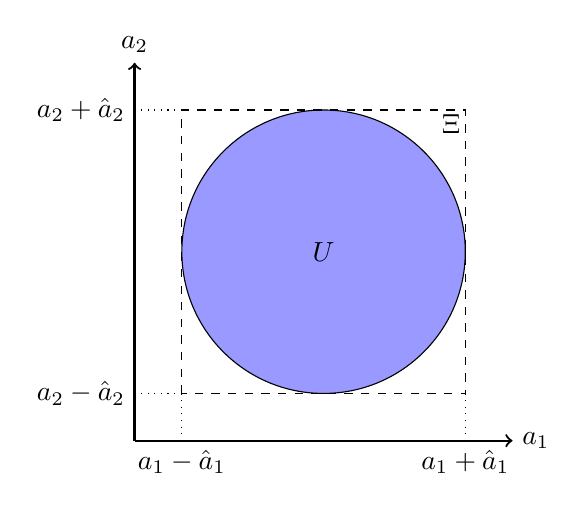
\begin{tikzpicture}[scale = 1.2]
		% Uncertainty set
		\filldraw[fill=blue!40!white] (2,2) circle (1.5cm);
%			\draw[help lines] (0,0) grid (4,4);
		\draw[dashed] (0.5,0.5) rectangle (3.5,3.5);
		\draw[thick, ->] (0,0) -- (0,4);
		\draw[thick, ->] (0,0) -- (4,0);
		\node[right] at (4,0) { $a_1$};
		\node[above] at (0,4) { $a_2$}; 
		\draw[dotted] (0.5,0.5) -- (0.5,0) node[below] { $a_1 - \hat{a}_1$}; 
		\draw[dotted] (3.5,0.5) -- (3.5,0) node[below] { $a_1 + \hat{a}_1$};
		\draw[dotted] (0.5,0.5) -- (0,0.5) node[left] { $a_2 - \hat{a}_2$}; 
		\draw[dotted] (0.5,3.5) -- (0,3.5) node[left] { $a_2 + \hat{a}_2$};
		\node[below left] at (3.55,3.55) {$\Xi$};
		\node at (2,2) {$U$};
	\end{tikzpicture}

\end{frame}


\begin{frame}{Uncertainty set geometries}{Polyhedral uncertainty set \cite{bertsimas2004price}}

	\begin{itemize}
		\item Allows for controlling conservatism;
		\item Retains problem complexity;
		\item \alert{Budget of uncertainty} lacks interpretability.
	\end{itemize}
	
	The \alert{uncertainty set} is
	$$
		U_i = \braces{\eta_i : ||\eta_i||_1 \le \Gamma_i} \equiv \braces{\eta_{ij} : \sum_{j \in J_i} \eta_{ij} \le \Gamma_i, \forall j \in J_i}.
	$$
	
	\pause
	The \alert{lower-level problem} becomes
	%
	\begin{equation*}
		\maxi_{\eta_i \in U_i}\braces{\sum_{j \in J_i} \eta_{ij}\hat{a}_{ij}x_j : \sum_{j \in J_i} \eta_{ij} \le \Gamma_i, \ 0 \le \eta_{ij} \le 1, \ \forall j \in J_i}.
	\end{equation*}
	
\end{frame}


\begin{frame}{Uncertainty set geometries}{Polyhedral uncertainty set \cite{bertsimas2004price}}

	In this case, the lower-level problem does not admit a closed form.  However, it is a \alert{linear program}. 
	\vspace{-6pt}
	\begin{itemize}
		\item Strong duality (primal-dual equivalence) is available;
		\item True for any \alert{convex}%
		\footnote{Satisfying some constraint qualification.}
		%
		 lower-level problem.	
	\end{itemize}
	%
	\pause
	\begin{equation*}
		\begin{split}
			\maxi_{\eta_i \in U_i} & \sum_{j \in J_i} \eta_{ij} \hat{a}_{ij}x_j \\
			 \st & \sum_{j \in J_i} \eta_{ij} \le \Gamma_i \ (\pi_i) \\
			 & 0 \le \eta_{ij} \le 1, \ (p_{ij}) \ \forall j \in J_i
		\end{split}
		\ \Rightarrow \
		\begin{split}
			\mini_{\pi_i, p_i} & \Gamma_i\pi_i + \sum_{j \in J_i} p_{ij} \\
			 \st & \pi_i + p_{ij} \ge \hat{a}_{ij}x_j, \forall j \in J_i \\
			 &p_{ij} \ge 0, \ \forall j \in J_i \\
			 &\pi_i \ge 0.
		\end{split}
	\end{equation*}
	
\end{frame}


\begin{frame}{Uncertainty set geometries}{Polyhedral uncertainty set \cite{bertsimas2004price}}

	\centering
	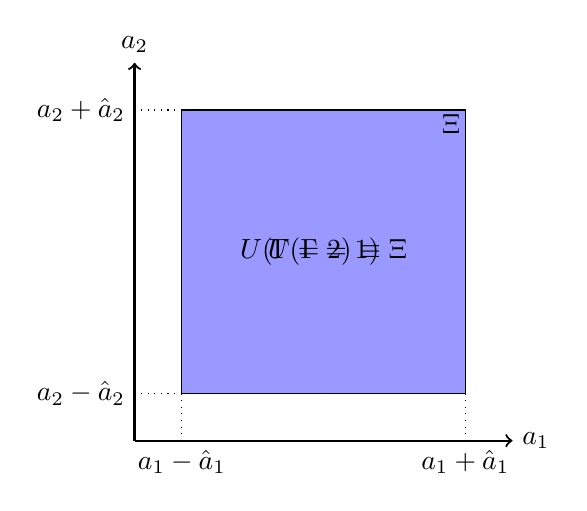
\begin{tikzpicture}[scale = 1.2]
		% Uncertainty set
		\uncover<1>{\filldraw[fill=blue!40!white] (2,0.5) -- (3.5,2) -- (2,3.5) -- (0.5, 2) -- cycle;}
		\uncover<2->{\filldraw[fill=blue!40!white] (0.5,0.5) rectangle (3.5,3.5);}
%			\draw[help lines] (0,0) grid (4,4);
		\draw[dashed] (0.5,0.5) rectangle (3.5,3.5);
		\draw[thick, ->] (0,0) -- (0,4);
		\draw[thick, ->] (0,0) -- (4,0);
		\node[right] at (4,0) { $a_1$};
		\node[above] at (0,4) { $a_2$}; 
		\draw[dotted] (0.5,0.5) -- (0.5,0) node[below] { $a_1 - \hat{a}_1$}; 
		\draw[dotted] (3.5,0.5) -- (3.5,0) node[below] { $a_1 + \hat{a}_1$};
		\draw[dotted] (0.5,0.5) -- (0,0.5) node[left] { $a_2 - \hat{a}_2$}; 
		\draw[dotted] (0.5,3.5) -- (0,3.5) node[left] { $a_2 + \hat{a}_2$};
		\uncover<1>{\node[below left] at (3.55,3.55) {$\Xi$};}
		\uncover<1>{\node at (2,2) {$U(\Gamma = 1)$};}
		\uncover<2->{\node at (2,2) {$U(\Gamma = 2) \equiv \Xi$};}
	\end{tikzpicture}

\end{frame}


\begin{frame}{Robust counterparts}

	Let us consider a knapsack problem of the form
	%
	\begin{equation*}
	\begin{aligned}
		\mini & c^\top x \\		
		\text{s.t.:~} & \sum_{j \in [n]} a_j x_j \le b \\
		& 0 \le x_j \le 0, \ \forall j \in [n].
	\end{aligned}
	\end{equation*}
	
	\pause
	The \alert{robust counterparts} for the previous uncertainty sets are:
	\begin{columns}
	\column{0.4\textwidth}
		\begin{block}{Box}
			\vspace{-12pt}
			\begin{equation*}
			\begin{aligned}
				\mini & c^\top x \\		
				\text{s.t.:~} & \sum_{j \in [n]} (a_j + \hat{a}_{ij})x_j \le b \\
				& 0 \le x_j \le 1, \ \forall j \in [n].
			\end{aligned}
			\end{equation*}
		\end{block}
	\column{0.45\textwidth}
		\begin{block}{Ellipsoid}
			\vspace{-12pt}
			\begin{equation*}
			\begin{aligned}
				\mini & c^\top x \\		
				\text{s.t.:~} & \sum_{j \in [n]} a_j x_j + \Gamma\sqrt{\sum_{j \in [n]} (\hat{a} x_j)^2} \le b \\
				& 0 \le x_j \le 1, \ \forall j \in [n].
			\end{aligned}
			\end{equation*}
		\end{block}
	\end{columns}

\end{frame}


\begin{frame}{Robust counterparts}

	Let us consider a knapsack problem of the form
	%
	\begin{equation*}
	\begin{aligned}
		\mini & c^\top x \\		
		\text{s.t.:~} & \sum_{j \in [n]} a_j x_j \le b \\
		& 0 \le x_j \le 1, \ \forall j \in [n].
	\end{aligned}
	\end{equation*}
	
	The \alert{robust counterparts} for the previous uncertainty sets are:
	
	\begin{block}{Polyhedral} 
		\vspace{-18pt}
		\begin{equation*}
		\begin{aligned}
			\mini & c^\top x \\		
			\text{s.t.:~} & \sum_{j \in [n]} a_j x_j + \Gamma \pi + \sum_{j \in [n]} p_j \le b \\
			& \pi + p_j \ge \hat{a}_j x_j, \ \forall j \in [n] \\
			& 0 \le x_j \le 1, p_j \ge 0, \ \forall j \in [n] \\
			& \pi \ge 0.
		\end{aligned}
		\end{equation*}
	\end{block}
	
\end{frame}


\begin{frame}{On constraint violation probabilities}

	Arguably, \alert{Bertsimas \& Sim (2004)} raised attention to robust optimisation with ``the price of robustness''.
	\vspace{-6pt}
	\begin{itemize}
		\item The \alert{price} refers to the optimality traded off for feasibility guarantees;
		\item Quantifying these trade-offs can be done:
		\begin{enumerate}
			\item Using \alert{theoretical} bounds;
			\item Via \alert{simulating} solution performance.	
		\end{enumerate}
		\item In my own experience, theoretical bounds are often loose. 	
	\end{itemize}
	
	\pause
	For example, {\small \cite{bertsimas2004price}} show the probability of violation of constraint $i \in [m]$ to be
	\begin{equation*}
		P^{\text{vio}} = P\left(a_{ij}x_j + \max_{\eta_i \in U_i} \braces{\sum_{j \in J_i}\eta_{ij}\hat{a}_{ij}x_j} > b_i\right) \le e^{\frac{-\Gamma^2}{2|J_i|}},
	\end{equation*}	
	%where $\Delta = 1$ for box sets, and $\Gamma$ for ellipsoidal and polyhedral sets.
	
\end{frame}


\section{Adjustable robust optimisation}


\begin{frame}{Multi-stage robust optimisation}

	We focus on 2-stage adjustable robust optimisation (ARO) problems:
	\begin{equation} \tag{ARO}
	\begin{aligned}
		\min~  & c^\top x + \max_{\xi \in U \subset \Xi} \min_y q^\top y(\xi) \\
		\text{s.t.:~}  & Ax = b, \ x \ge 0 \\
			   & T(\xi)x + Wy(\xi) = h(\xi), \ \forall \xi \in U \subset \Xi \\
			   & y(\xi) \ge 0, \ \forall \xi \in \Xi.
	\end{aligned}
	\end{equation}
	\pause
	\vspace{-6pt}
	\begin{itemize}
		\item Only \alert{RHS} uncertainty: $T(\xi) = T$, $W(\xi) = W$, and $q(\xi) = q$ $\forall \xi \in \Xi$;
		\item Assumption often necessary to eliminate \alert{quadratic} dependence between $\xi$ and decision variables;
		\item Not necessary if the uncertainty set is \alert{discrete} and \alert{finite} (scenarios)
	\end{itemize}



	
\end{frame}


\begin{frame}{A side note: min-max, minimum regret and related}

If the uncertainty set is a finite and discrete set of scenarios, we have that 
%
\begin{align*}
	\mini_x & c^\top x + \maxi_{s \in U} \mini_{y}q_s^\top y_s \\
	\text{s.t.: } & T_sx + W_s y_s \le h_s, \ \forall s \in U \\
	& x \in X
\end{align*}
%
is a \alert{tractable} ARO \cite{mulvey1995robust}. \pause Variants include:

\vspace{-12pt}
\begin{columns}
\column[t]{0.45\textwidth}
	\begin{block}{Min-max}
	\vspace{-18pt} 
		\begin{align*}
			\mini_x & c^\top x + \theta \\
			& \theta \ge q_s^\top y_s, \ \forall s \in U \\
			\text{s.t.: } & T_s x + W_s y_s \le h_s, \ \forall s \in U \\
			& x \in X
		\end{align*}
	\end{block}	
\column[t]{0.45\textwidth}
		\begin{block}{Min-regret}
	\vspace{-18pt} 
		\begin{align*}
			\mini_x & c^\top x + \theta \\
			& \theta \ge q_s^\top y_s - q_s^\top y^\star_s, \ \forall s \in U \\
			\text{s.t.: } & T_sx + W_s y_s \le h_s, \ \forall s \in U \\
			& x \in X
		\end{align*}
		
		\vspace{-12pt}
		where $y^\star_s$ is optimal for $s \in U$.
	\end{block}	
\end{columns}
	
\end{frame}


\begin{frame}{Affinely adjustable robust optimisation {\small \cite{ben2004adjustable}}}

	One idea for modelling adjustability is using \alert{affine policies}:
	\vspace{-6pt}
	\begin{itemize}
		\item Replace $y(\xi)$ with $\alpha + \beta \xi$;
		\item $h(\xi)$ is assumed \alert{affinely dependent} on $\xi$, e.g.: $h(\xi)	 = h + \hat{h}\xi$.
	\end{itemize}
	
	\pause
	Then ARO becomes:
	\begin{equation*}
	\begin{aligned}
		\mini_{x, \alpha, \beta}~  & c^\top x + \theta  \\
		\text{s.t.:~}  & \theta \ge q^\top (\alpha + \beta \xi), \ \forall \xi \in U \\
			   & Ax = b, \ x \ge 0 \\
			   & Tx + W(\alpha + \beta \xi) \le h(\xi), \ \forall \xi \in U \\
			   & y(\xi) \ge 0, \ \forall \xi \in \Xi.
	\end{aligned}
	\end{equation*}
	\pause
	Similar to the static case, computational \alert{tractability} can be achieved:
		\vspace{-6pt}
		\begin{itemize}
			\item Requires that $U$ is a box or ellipsoidal set;
			\item For a practical example, see {\small \cite{ben2005retailer}}	
		\end{itemize}
   
\end{frame}


\begin{frame}{Adjustable robust optimisation}
	
	An \alert{alternative} approach: looking closer at the inner problem as a \alert{bilevel} optimisation problem.
	
	Let us restate our ARO in a simplified notation. For that, let
	\vspace{-6pt} 
	\begin{itemize}
		\item $X = \braces{x \in \reals^{n_1} : Ax = b, x \ge 0}$;
		\item $Y = \braces{y \in \reals^{n_2} : y \ge 0}$;
		\item Uncertainty in \alert{RHS only}, with $h(\xi) = h - \hat{h}\xi$, and $\xi \in \brackets{\, \underline{\xi}, \overline{\xi}\,}$
	\end{itemize} 
	
	\pause
	Then we have that ARO is equivalent to
	
	\begin{equation} \tag{ARO}
		\min_{x \in X} c^\top x + \mathcal{Q}(x),
	\end{equation}

	where
	\begin{equation*}
		\mathcal{Q}(x) = \braces{\maxi_{\xi \in U}\mini_{y \in Y} q^\top y : Tx =(h - \hat{h}\xi) - Wy}.
	\end{equation*}
	
\end{frame}


\begin{frame}{Adjustable robust optimisation \& CCG}

	Let us assume that an \alert{oracle} is available such that, for a given $\overline{x} \in X$ it evaluates $\mathcal{Q}(x)$ and returns associated $(\overline{\xi}, \overline{y})$, if they exist.
	
	\pause
	In addition, let us assume that the uncertainty set is \alert{finitely} representable:
	\vspace{-6pt}
	\begin{itemize}
		\item Scenarios, but an \alert{intractable amount} of them (e.g., samples, or data)
		\item \alert{Polyhedral} set (finite extreme points and rays)	
	\end{itemize}
	
	\pause
	In that case, we can employ \alert{column-and-constraint generation} (CCG) {\small \cite{zeng2013solving}} to solve ARO: 
	
	\vspace{-12pt}
	\begin{columns}
	\column[t]{0.43\textwidth}
	\begin{block}{Main problem $M^k$: $\overline{x}^{k+1}$} \small 
	
	\vspace{-21pt}
	\begin{align*}
		\mini_{x,y,\theta} & c^\top x + \theta \\
		& \theta \geq q^\top y_l, \ l \in [k] \\
		& x \in X \\ 
		& Tx = h - \hat{h} \overline{\xi}_l - Wy_l, \  l \in [k] \\
		& y_l \in Y, \ l \in [k].
	\end{align*}
	\end{block}

	\column[t]{0.45\textwidth}
	\begin{block}{Oracle $\mathcal{Q}(\overline{x}^{k+1})$: $\overline{\xi}^{k+1}$} \small 
	
	\vspace{-21pt}
	\begin{align*}
		\maxi_{\xi \in U} \mini_{y \in Y}~ & q^\top y \\
		\text{s.t.:~} & T\overline{x}^{k+1} = (h - \hat{h}\xi) - Wy.
	\end{align*}
	\end{block}		
	\end{columns}
	
\end{frame}


\begin{frame}{Adjustable robust optimisation \& CCG}

	In summary, the CCG method can be stated as
	\begin{enumerate}[<+->]
		\item {\bf Initialisation.} $LB = -\infty$, $UB = \infty$, $k = 0$.
		\item {\bf Solve the main problem $M^k$.} Let $\underline{z}^k = c^\top x^k + \theta^k$, where $\argmin M^k = (x^k, \theta^k, (y_l^k)_{l=1}^k)$. Make $LB = \underline{z}^k$.
	\item {\bf Solve $\mathcal{Q}(x^k)$}. Let $\argmin \mathcal{Q}(x^k)=(\overline{\xi}^{k+1}, \overline{y}^{k+1})$, if it exists. Let $\overline{z}^{k} = c^\top x^k + \mathcal{Q}(x^k)$. Make  $UB = \min\braces{UB, \overline{z}^{k}}$. {\bf If} $UB = LB < \epsilon$, {\bf return $x^k$}.
	\item {\bf Add column and constraints to $M^k$.} If $\mathcal{Q}(x^k)$ is feasible, create columns $y_{k+1}$ and, together with the constraints
		\begin{align}
			& \theta \geq q^\top y_{k+1} \\
			& Tx = h - \hat{h} \overline{\xi}_{k+1} - Wy_{k+1}, \ y_{k+1} \in Y,	 \label{eq:feas_cut}	
		\end{align}
  	add them to $M^k$, forming $M^{k+1}$. Make $k = k+1$ and return to {\color{blue}Step 2}. If $\mathcal{Q}(x^k)$ is not feasible, then only \eqref{eq:feas_cut} is created.
\end{enumerate}
	
\end{frame}


\begin{frame}{Adjustable robust optimisation \& CCG}{Practical remarks}

	Essentially, CCG for ARO is a \alert{delayed-generation} approach of the min-max formulation
	\begin{itemize}
		\item Can thus be useful when \alert{too many scenarios} are available;
		\item Convergence relies on a \alert{finiteness argument} on the uncertainty set.	
	\end{itemize}
	
	\pause
	CCG can be seen as a \alert{primal equivalent} to Benders decomposition
	\begin{itemize}
		\item One can use the same column generation approach in the context of the L-shaped method {\small \cite{van1969shaped}};
		\item This can help as a way to \alert{transmit} ``recourse information'' to the main problem.	
	\end{itemize}

\end{frame}


\begin{frame}{Adjustable robust optimisation \& CCG}{On solving $\mathcal{Q}(x)$}

	Recall that $\mathcal{Q}(x)$  is of the form
	\begin{align*}
	\mathcal{Q}(x)	 = &\max_u q^\top y    \\
	   \st &u \in \mathcal{U}  \\ 	 
		   &y \in \argmin_y q^\top y \\
	       &\qquad \quad \text{s.t.:~} Tx = h - \hat{h} \xi - Wy \\
	       &\qquad \quad \phantom{~\text{s.t.:~}} y \in Y. 
	\end{align*}
	%
	\pause
	This is a \alert{bilevel model} and can be solved using dedicated methods.
	\vspace{-6pt}
	\begin{itemize}
		\item Most techniques rely on \alert{posing optimality conditions} of the lower-level problem to yield an \alert{equivalent single-level} (tractable) problem;
		\item Thus, \alert{lower-level convexity} (plus CQ) is often a requirement.
	\end{itemize}

\end{frame}


\begin{frame}{Adjustable robust optimisation \& CCG}{On solving $\mathcal{Q}(x)$}

	Example: assume that $Y = \reals_+^{n_2}$. We can use strong duality to reformulate the lower-level problem, obtaining
	%
	\begin{align*}
		\mathcal{Q}(x) = &\max_{\xi,\pi} (h - \hat{h} \xi - Tx)^\top \pi \\
		   \text{s.t.:~} & \pi^\top W \leq q^\top \\
		   	   & \xi \in U.	 
	\end{align*}
	%
	\pause
	$\mathcal{Q}(x)$ is solvable, if:
	\vspace{-6pt} 
	\begin{enumerate}
		\item $\xi$ is integer or has a discrete domain, since $\xi^\top \pi$ can be reformulated exactly (e.g., {\small \cite{rintamaki2023achieving}});
		\item if $-(\hat{h}\xi)^\top \pi + (h - Tx)^\top \pi$ is a \alert{concave bilinear} function in $\pi$ and $\xi$;
		\item if applying a \alert{global solver} (e.g., Gurobi's spatial branch-and-bound method) is feasible from a computational standpoint.	
	\end{enumerate}

	
\end{frame}

\begin{frame}[allowframebreaks]{References}
	\bibliographystyle{apalike}
	\bibliography{../aux/references.bib}
\end{frame}

